\chapter{Initial Multi-Modelling using VDM}
\label{sec:initial}

In this section we provide guidance on producing initial multi-models from architectural descriptions produced using the INTO-CPS SysML profile. We focus on using discrete-event (DE) models to produce initial, abstract FMUs that allow integration testing through co-simulation before detailed modelling work is complete. This is called a ``DE-first'' approach~\cite{Fitzgerald&13b,Fitzgerald&13a}. We describe the use of VDM and the Overture tool, with FMI export plug-in installed, for this approach. The principles outlined in this section can be applied in other modelling tools. This approach can work with or without the SysML profile.

%In future, these guidelines will be expanded to include how and when to continuous-time (CT) formalisms in initial modelling.

%\section{Context}
\section{The DE-first Approach}

\begin{figure}[p]
\centering
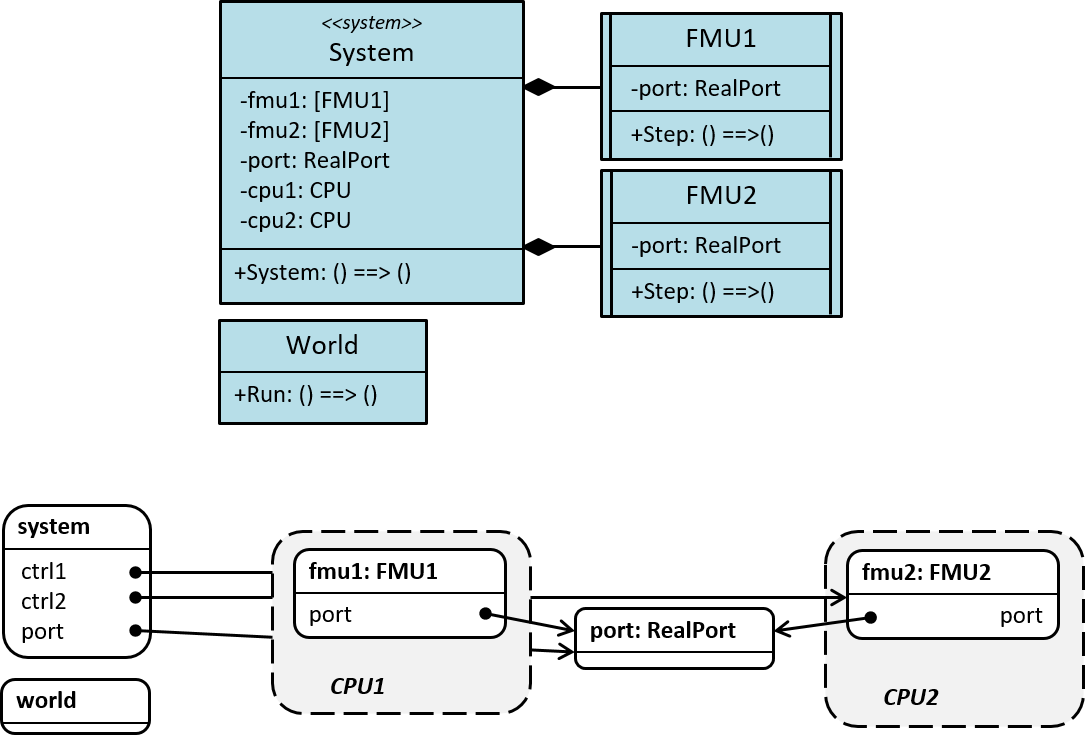
\includegraphics[scale=0.47]{figures/defirst_class}
\caption{Class diagram showing two simplified FMU classes created within a single VDM-RT project, and an object diagram showing them being instantiated as a test.}
\label{fig:defist_class}
\end{figure}

\begin{figure}[p]
\centering
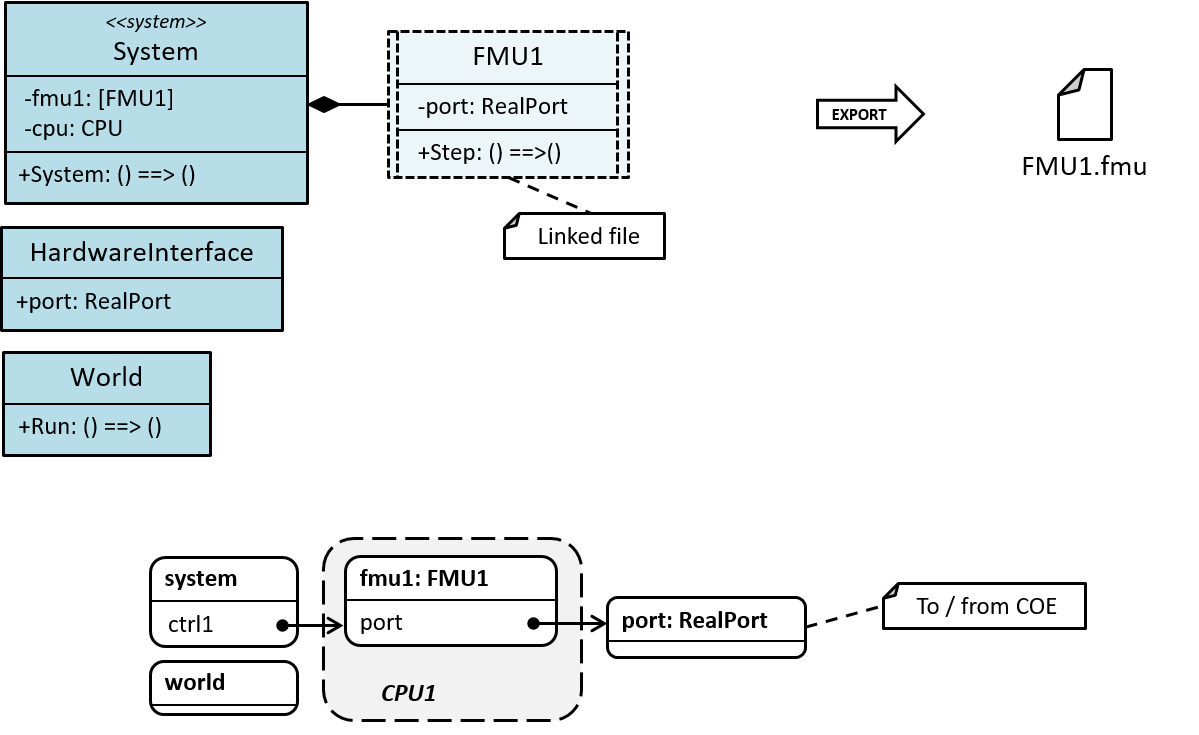
\includegraphics[scale=0.47]{figures/defirst_fmu1}
\caption{Class and object diagrams showing a linked class within its own project for FMU creation.}
%\begin{center}
%\subfigure[Structure of the FMU1 project]
%{
%	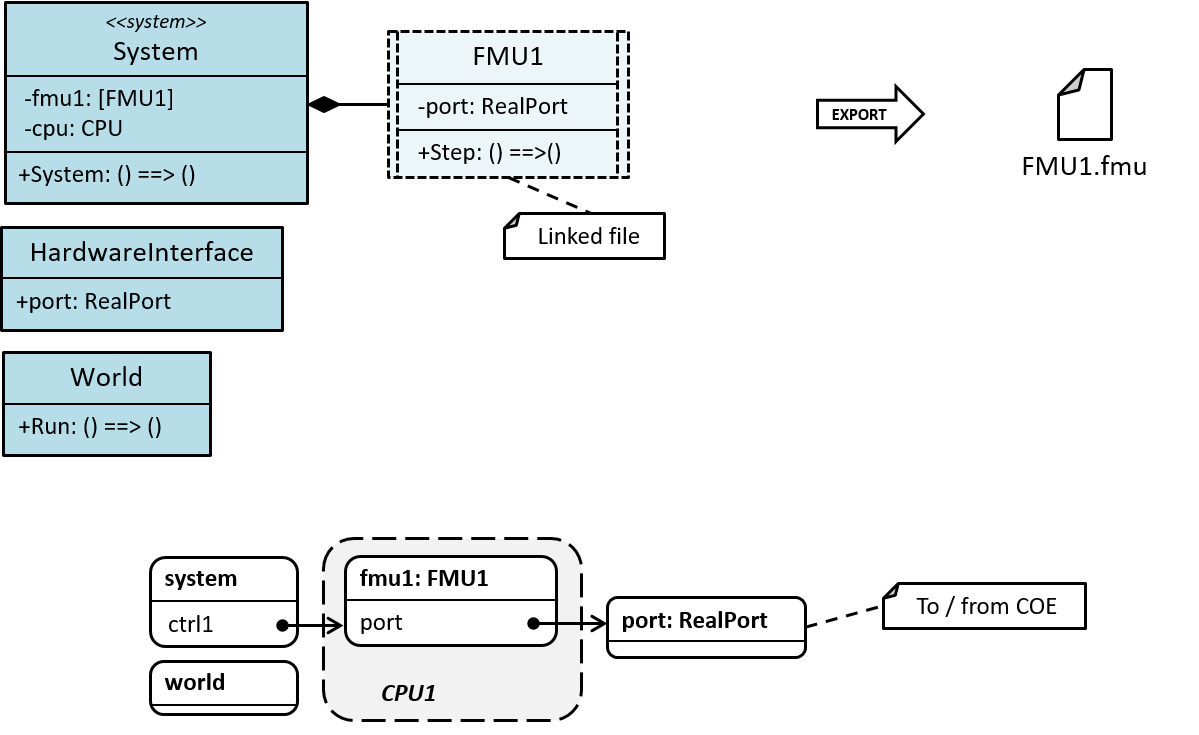
\includegraphics[scale=0.4]{figures/defirst_fmu1}
%	\label{fig:snd_rec}
%}
%\subfigure[Structure of the FMU2 project]
%{
%	\includegraphics[scale=0.4]{figures/defirst_fmu2}
%	\label{fig:snd_ether_rec}
%}
%\caption{Class diagrams showing the FMU classes being included (through file linking) in their own projects ready for export to FMU}
\label{fig:defirst_fmus}
\end{figure}

After carrying out requirements engineering (RE), as described in Chapter~\ref{sec:reqeng}, and design architectural modelling in SysML, as described in Chapter~\ref{sec:sysml}, the engineering team should have the following artifacts available:

\begin{itemize}[noitemsep]
\item One or more Architecture Structure Diagrams (ASDs) defining the composition of\\ \texttt{<<EComponent>>}s (to be realised as \texttt{<<Cyber>>} or \texttt{<<Physical>>} FMUs) that will form the multi-model.
\item Model descriptions exported for each \texttt{<<EComponent>>}.
\item One or more Connections Diagrams (CDs) that will be used to configure a multi-model.
\end{itemize}

The next step is to generate a multi-model configuration in the INTO-CPS Application and populate it with FMUs, then run a first co-simulation. This however requires the source models for each FMU to be ready. If they already exist this is easy, however they may not exist if this is a new design. In order to generate these models, the model descriptions for each \texttt{<<EComponent>>} can be passed to relevant engineering teams to build the models, then FMUs can be passed back to be integrated.

It can be useful however to create and test simple, abstract FMUs first (or in parallel), then replace these with higher-fidelity FMUs as the models become available. This allows the composition of the multi-model to be checked early, and these simple FMUs can be reused for regression testing. This approach also mitigates the problem of modelling teams working at different rates.

Where these simple FMUs are built within the DE formalism (such as VDM), this is called a \emph{DE-first} approach. This approach is particularly appropriate where complex DE control behaviours ---such as supervisory control or modal behaviours--- are identified as a priority or where the experience of the modelling team is primarily in the DE domain~\cite{Fitzgerald&14c}.

Guidance on how to produce DE approximations for use in multi-modelling, and in particular approximations of CT behaviour, can be found in material describing the Crescendo baseline technology~\cite{Fitzgerald&13a}, which is also available via the Crescendo website\footnote{See \url{http://crescendotool.org/documentation/}}.

\section{DE-first within INTO-CPS}

Given an architectural structure diagram, connections diagram and model descriptions for each \texttt{<<EComponent>>}, the suggested approach is to begin by building a single VDM-RT project in Overture with the following elements:

\begin{itemize}[noitemsep]
\item A class for each \texttt{<<EComponent>>} representing an FMU. Each class should define port-type instance variables (i.e. of type \texttt{IntPort}, \texttt{RealPort}, \texttt{BoolPort}, or \texttt{StringPort}) corresponding to the model description and a constructor to take these ports as parameters. Each FMU class should also define a thread that calls a \texttt{Step} operation, which should implement some basic, abstract behaviour for the FMU.
\item A \texttt{system} class that instantiates port and FMU objects based on the connections diagram. Ports should be passed to constructor of each FMU object. Each FMU object should be deployed on its own CPU.
\item A \texttt{World} class that starts the thread of each FMU objects.
\end{itemize}

Class and object diagrams giving an example of the above is shown in Figure~\ref{fig:defist_class}. In this example, there are two \texttt{<<EComponent>>}s (called \emph{FMU1} and \emph{FMU2}) joined by a single connection of type real. Such a model can be simulated within Overture to test the behaviour of the FMUs. This approach can be combined with the guidance in Chapter~\ref{sec:networks} to analyse more complicated networked behaviour. Once the behaviour of the FMU classes has been tested, actual FMUs can be produced and integrated into a first multi-model by following the guidance below.

\section{FMU Creation}

The steps outlined below assume a knowledge of FMU export in Overture, which can be found in the User Manual, Deliverable D4.3a~\cite{INTOCPSD4.3a}, in Section 5.1. To generate FMUs, a project must be created for each \texttt{<<EComponent>>} with:

\begin{itemize}[noitemsep]
\item One of the FMU classes from the main project.
\item A \texttt{HardwareInterface} class that defines the ports and annotations required by the Overture FMU export plug-in, reflecting those defined in the model description.
\item A \texttt{system} class that instantiates the FMU class and passes the port objects from the \texttt{HardwareInterface} class to its constructor.
\item A \texttt{World} class that starts the thread of the FMU class.
\end{itemize}

The above structure is shown in Figure~\ref{fig:defirst_fmus}. A skeleton project with a correctly annotated \texttt{HardwareInterface} class can be generated using the model description import feature of the Overture FMU plug-in. The FMU classes can be linked into the projects (rather than hard copies being made) from the main project, so that any changes made are reflected in both the main project and the individual FMU projects. These links can be created by using the \emph{Advanced} section of the \emph{New \textgreater\ Empty VDM-RT File} dialogue, using the \texttt{PROJECT-1-PARENT\_LOC} variable to refer to the workspace directory on the file system (as shown in Figure~\ref{fig:defirst_link}). Note that if the FMU classes need to share type definitions, these can be created in a class called \texttt{Types} in the main project, then this class can be linked into each of the FMU projects in the same way.

From these individual project, FMUs can be exported and co-simulated within the INTO-CPS tool. These FMUs can then be replaced as higher-fidelity versions become available, however they can be retained and used for regression and integration testing by using different multi-model configurations for each combination.

\begin{figure}
\centering
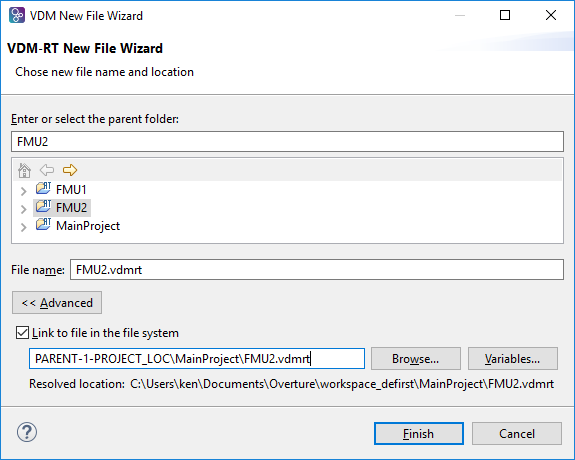
\includegraphics[scale=0.8]{figures/defirst_link}
\caption{Linking files in the \emph{New \textgreater\ Empty VDM-RT File} dialogue.}
\label{fig:defirst_link}
\end{figure}

\begin{figure}
\centering
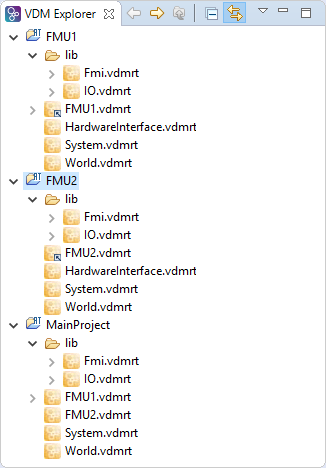
\includegraphics[scale=0.8]{figures/defirst_workspace}
\caption{Project structure of an Overture workspace showing a main project and two projects used for generating FMUs from linked class files.}
\label{fig:defirst_workspace}
\end{figure}


%\begin{figure}
%\centering
%\includegraphics[scale=0.4]{figures/defirst_object}
%\caption{Object showing two controllers being simulated within a main project, and being co-simulated in their own FMUs}
%\label{fig:defist_object}
%\end{figure}

